\documentclass[9pt,a4paper,twocolumn]{extarticle}

% Journal-style reconstruction based on the supplied six-page DU sample.
% Unlike the exact-copy source, this file is fully editable LaTeX.
\usepackage[a4paper,top=1.45cm,bottom=1.45cm,left=1.55cm,right=1.55cm,headheight=16pt,headsep=6pt,footskip=17pt]{geometry}
\usepackage[T1]{fontenc}
\usepackage[utf8]{inputenc}
\usepackage{lmodern}
\usepackage{microtype}
\usepackage{graphicx}
\usepackage{booktabs,tabularx,array,multirow}
\usepackage{amsmath,amssymb}
\usepackage{caption}
\usepackage{fancyhdr}
\usepackage{xcolor}
\usepackage{titlesec}
\usepackage{enumitem}
\usepackage{tikz}
\usepackage{xurl}
\usepackage{url}
\usepackage[hidelinks]{hyperref}
\usepackage{placeins}
\usepackage{float}
\usetikzlibrary{arrows.meta,positioning,shapes.geometric}

\definecolor{navy}{RGB}{34,59,99}
\definecolor{lightblue}{RGB}{235,241,249}
\definecolor{midblue}{RGB}{81,112,158}
\hypersetup{colorlinks=true,linkcolor=navy,citecolor=navy,urlcolor=navy}
\setlength{\columnsep}{0.55cm}
\setlength{\parindent}{1em}
\setlength{\parskip}{1.5pt}
\setlist{nosep,leftmargin=1.2em}
\captionsetup{font=footnotesize,labelfont=bf,justification=raggedright,singlelinecheck=false}
\titleformat{\section}{\bfseries\color{navy}\fontsize{10}{11}\selectfont}{\thesection}{0.45em}{}
\titleformat{\subsection}{\bfseries\itshape\fontsize{9}{10}\selectfont}{\thesubsection}{0.4em}{}
\titlespacing*{\section}{0pt}{5pt}{2pt}
\titlespacing*{\subsection}{0pt}{4pt}{1pt}
\pagestyle{fancy}
\fancyhf{}
\setlength{\headheight}{16pt}
\setlength{\headsep}{6pt}
\setlength{\footskip}{17pt}
\renewcommand{\headrulewidth}{0pt}
\renewcommand{\footrulewidth}{0pt}
\setlength{\fboxsep}{0pt}
\fancyhead[L]{%
  \hspace*{-1cm}\makebox[\dimexpr\textwidth+1cm\relax][l]{%
    \colorbox{navy}{%
      \parbox[c][14pt][c]{\dimexpr\textwidth+1cm\relax}{%
        \hspace{6pt}\scriptsize\bfseries\color{white}%
        B.Sc. (Hons.) Computer Science | Semester V | Ramanujan College, University of Delhi%
        \hfill Machine Learning Assignment\hspace{6pt}%
      }%
    }%
  }%
}
\fancyfoot[L]{\scriptsize\color{gray}Problem No. 4 -- District-wise seasonal crop-production case study}
\fancyfoot[R]{\scriptsize\color{gray}Page \thepage}
\setcounter{secnumdepth}{3}
\newcommand{\keywords}[1]{\par\vspace{2pt}\noindent\textbf{Keywords:} #1}
\newcommand{\smallurl}[1]{\url{#1}}

\begin{document}
\sloppy

% Full-width title and abstract, matching the sample's first-page hierarchy.
\twocolumn[{
\begin{@twocolumnfalse}
\begin{center}
{\Large\bfseries\color{navy} Clustering Indian Districts by Seasonal Crop-Production Profiles Using Classical\\Machine-Learning Methods\par}
\vspace{5pt}
{\normalsize Radhika\par}
\vspace{2pt}
{\small Department of Computer Science, Ramanujan College, University of Delhi, New Delhi, India\\
University Roll No.: 24020570050 \;|\; E-mail: Radhika93962@gmail.com\\
Course: Machine Learning (B.Sc. (H) Computer Science, Semester V) \;|\; Supervisor: Dr. Nikhil Kumar Rajput\\
Problem No. 4 from ML Application Problems \;|\; Article type: Case Study}
\end{center}
\vspace{4pt}
\noindent\textbf{Abstract.} Agricultural planning is often designed around broad administrative categories, although districts can differ substantially in the seasonal distribution of cultivated area and crop production. This case study uses district-wise crop statistics from India to identify groups of districts with similar seasonal agricultural profiles. The supplied crop-production file contains 246,091 records and seven variables for 1997--2015. The primary analysis focuses on Kharif, Rabi and Whole Year crops and uses records from 1997--2014 because the 2015 file contains markedly fewer observations. Seasonal area shares are calculated at the state--district level. To create a crop-balanced production-composition feature, production is first normalised within each district--crop across the three seasons and then averaged across crops. Six resulting features are standardised and analysed using K-Means and agglomerative hierarchical clustering. The number of K-Means clusters is examined with the Elbow Method and Euclidean silhouette score for $k=2$--$10$. The maximum tested silhouette occurs at $k=2$ (0.4082). Among the compared methods, Ward agglomerative clustering gives the strongest Euclidean separation (silhouette 0.4615; Davies--Bouldin index 0.8936), while average-linkage cosine clustering gives a cosine silhouette of 0.5363. K-Means identifies two broad profiles: a larger group with substantial Kharif and Rabi area shares (538 districts) and a smaller group with substantial Kharif and Whole Year area shares (105 districts). The results are exploratory and can support further region-focused agricultural planning; they are not validated agro-ecological zones or causal classifications.
\keywords{India; crop production; seasonal cropping; district-level analysis; K-Means; hierarchical clustering; PCA; SDG 2; SDG 15}
\vspace{7pt}\hrule\vspace{5pt}
\end{@twocolumnfalse}
}]

\section{Introduction}
Agriculture in India is spatially heterogeneous. Rainfall regimes, irrigation access, soil conditions, crop choices and local infrastructure influence what farmers cultivate and when they cultivate it. A national or state-level summary can conceal differences between districts, even though district-level patterns are often the scale at which extension programmes and agricultural support are organised. Understanding these differences is therefore useful for describing agricultural systems and identifying areas that may benefit from more tailored planning.

Seasonal cropping patterns are one practical way to characterise this heterogeneity. Kharif crops are generally associated with the monsoon season, Rabi crops with the winter season, and Whole Year crops occupy a longer or year-round growing period in the source classification. Districts with similar seasonal distributions may face comparable planning questions, although similarity in these features does not imply identical soils, water availability or farmer circumstances.

Research on Indian crop distributions has shown that crop diversity and agricultural intensification vary across districts and regions. Smith, Ghosh and Hijmans [2] documented substantial spatial variation in crop diversity and changes in crop composition across India. Their work demonstrates why district-level patterns should not be hidden by national averages. A district-focused analysis of cropping patterns in West Bengal also highlights the relevance of local infrastructure, irrigation and climate when interpreting agricultural transitions [3].

The present study addresses the allocated Problem No. 4: to cluster districts by the share of area and production across Kharif, Rabi and Whole Year crops. Its objectives are: (i) to construct comparable district-level seasonal features; (ii) to examine the number of clusters using inertia and silhouette analysis; (iii) to compare K-Means with hierarchical clustering under Euclidean and cosine distances; and (iv) to describe the resulting groups using cluster profiles and a two-dimensional PCA projection. The work is framed as a descriptive case study for planners, not as a predictive model.

\section{Related Work}
District-level agricultural statistics have been used to study crop diversity, specialisation and transitions in cropping patterns. Smith et al. [2] analysed national and district-level crop distributions in India and reported that the direction of crop-diversity change differed across regions. This supports the use of spatially disaggregated evidence when discussing agricultural sustainability. In a regional study of West Bengal, the authors of [3] examined district-level cropping-pattern transitions and identified irrigation, climate and infrastructure as relevant contextual factors. These studies motivate a district-focused descriptive analysis, but they do not perform the same seasonal clustering task as the present assignment.

Clustering is an unsupervised learning approach that groups observations according to similarity in their feature representations. K-Means partitions observations by minimising within-cluster squared Euclidean distances [4]. Agglomerative hierarchical clustering builds nested groups by repeatedly merging observations or existing clusters; Ward's criterion selects merges that minimise the increase in within-cluster variance [5]. The silhouette coefficient measures how close an observation is to its own cluster relative to the nearest alternative cluster [6], while the Davies--Bouldin index summarises within-cluster scatter relative to between-cluster separation [7]. PCA is used here only to visualise the six-dimensional feature space in two dimensions [8].

\section{Dataset and Preprocessing}
\subsection{Source and description}
The project allocation specifies the Government of India's Open Government Data (OGD) resource, ``District-wise, season-wise crop production statistics from 1997'' [1]. The resource is attributed to the Directorate of Economics and Statistics, Department of Agriculture and Farmers Welfare, Ministry of Agriculture and Farmers Welfare. The official catalogue describes district-, crop-, season- and year-wise covered area and production statistics and identifies area in hectares and production in tonnes [1]. The supplied CSV is the Kaggle mirror named ``Crop Production in India'' and contains 246,091 rows and seven columns: State\_Name, District\_Name, Crop\_Year, Season, Crop, Area and Production. It covers 33 state/UT labels, 646 distinct district-name strings, 124 crops and crop years 1997--2015. Districts are identified by the combination of state and district name because district names alone are not unique.

\begin{table}[H]
\centering
\caption{Variables in the supplied crop-production file.}
\label{tab:variables}
\footnotesize
\begin{tabularx}{\columnwidth}{>{\raggedright\arraybackslash}p{0.30\columnwidth} X}
\toprule
\textbf{Variable} & \textbf{Description / use}\\
\midrule
State\_Name & State or Union Territory identifier\\
District\_Name & District label; paired with state\\
Crop\_Year & Year of the crop record\\
Season & Seasonal category; primary analysis uses three categories\\
Crop & Crop name used to form crop-level production shares\\
Area & Reported cultivated area; used for area shares\\
Production & Reported crop production; used for seasonal composition\\
\bottomrule
\end{tabularx}
\end{table}

\begin{figure}[H]
\centering
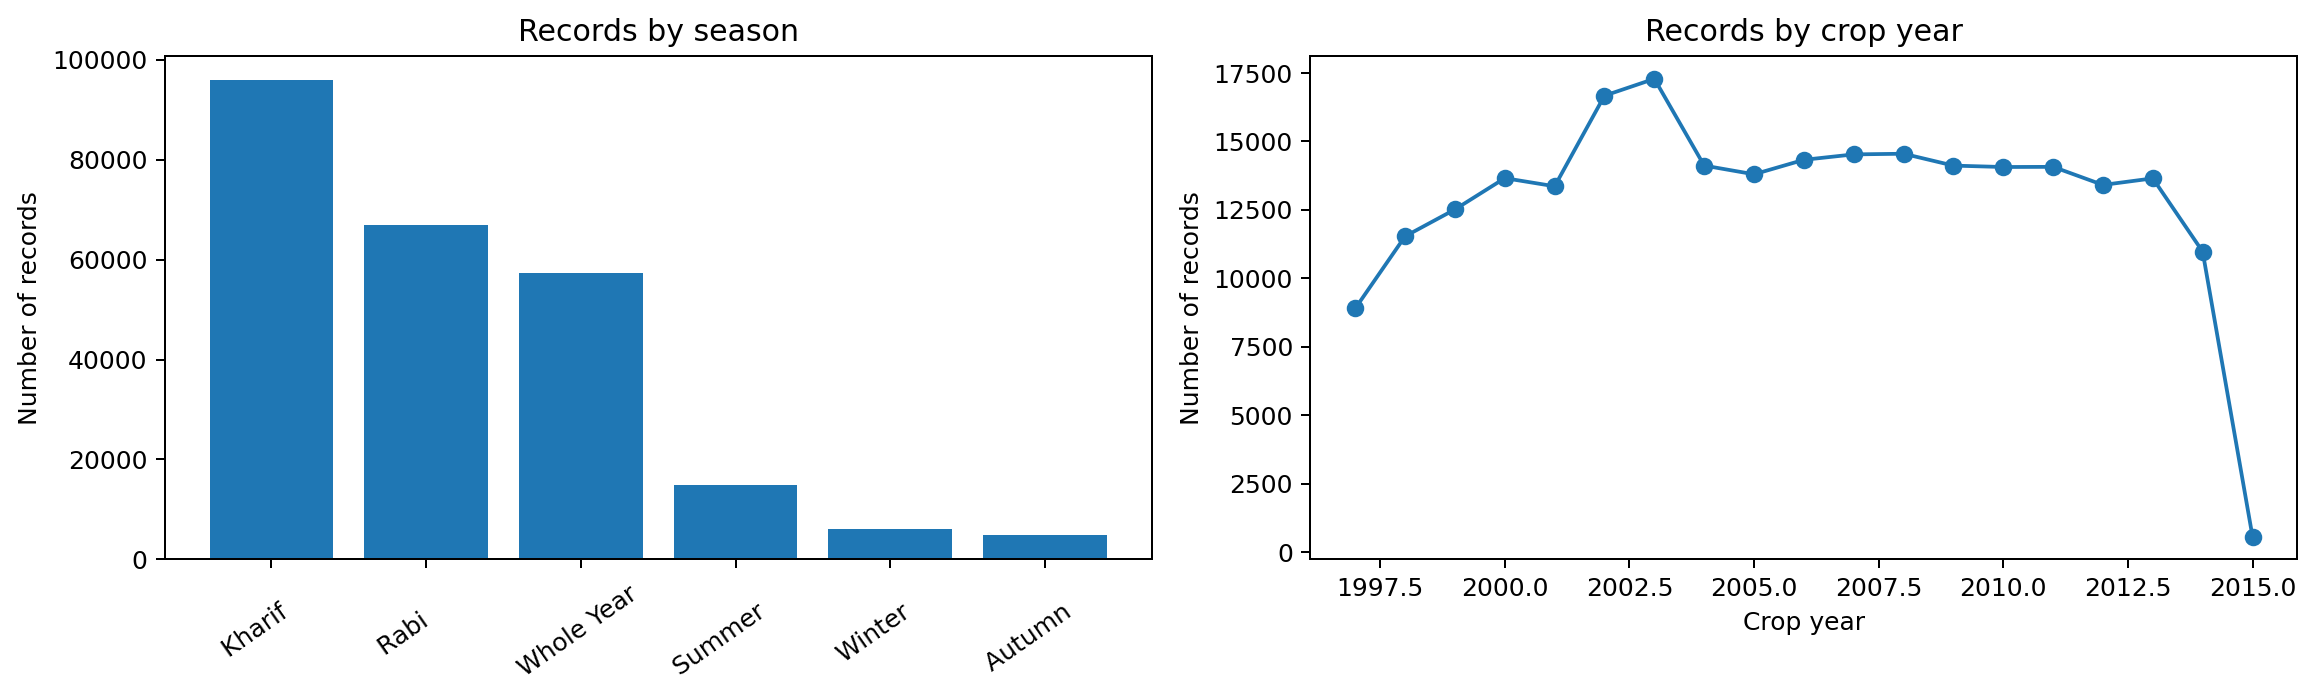
\includegraphics[width=\columnwidth]{00_dataset_overview.png}
\caption{Record coverage in the supplied file by season and crop year. The final year (2015) has markedly fewer records than preceding years.}
\label{fig:overview}
\end{figure}

\subsection{Cleaning and scope}
The raw file contains 3,730 missing Production values and no exact duplicate rows. Text fields were stripped of leading and trailing whitespace; Crop\_Year, Area and Production were converted to numeric values. The analysis retains crop years 1997--2014 and the three seasons named in the allocation: Kharif, Rabi and Whole Year. Autumn, Summer and Winter records are excluded from the primary analysis so that the feature space matches the assigned problem. The 2015 records are excluded because only 562 rows are present in that year, compared with 10,973 in 2014; this abrupt reduction indicates markedly incomplete coverage in the supplied file. This is a coverage-based analytical decision and does not mean that the official source ends in 2014.

Rows without state, district, crop, year or valid positive Area values are removed. Production features are calculated from non-missing, non-negative Production values. Districts represented in fewer than two of the three target seasons are excluded because their seasonal profiles are too incomplete for the intended comparison. After filtering, 220,208 crop records remain and 643 state--district units are retained for clustering; eight district units are excluded for insufficient seasonal coverage.

\subsection{Feature construction}
For each district $d$ and season $s$, area is summed across crops and years. The seasonal area share is
\begin{equation}
 A_{d,s}=\frac{\sum_{c,t} Area_{d,c,s,t}}{\sum_{s'}\sum_{c,t} Area_{d,c,s',t}}.
\label{eq:area}
\end{equation}
To prevent crops with large reported production magnitudes from dominating the district's production signature, production is first summed within each district--crop--season. For each district--crop pair, its production is normalised across the three seasons; these crop-level seasonal proportions are then averaged equally across crops in that district. The resulting $P_{d,s}$ is a crop-balanced seasonal production-composition feature, not the district's aggregate share of total tonnage. The six clustering variables are $A_{d,s}$ and $P_{d,s}$ for the three seasons. Both three-part compositions sum to approximately one for each retained district.

\section{Methodology}
\subsection{Standardisation and K-Means}
The six features are standardised using the feature-wise mean and standard deviation:
\begin{equation}
 z_{ij}=\frac{x_{ij}-\mu_j}{\sigma_j},
\end{equation}
where $x_{ij}$ is feature $j$ for district $i$, and $\mu_j$ and $\sigma_j$ are calculated across the 643 retained districts. Standardisation prevents features with larger numerical dispersion from dominating distance calculations.

K-Means assigns each district to one of $k$ clusters by minimising the within-cluster sum of squares:
\begin{equation}
 J=\sum_{r=1}^{k}\sum_{x_i\in C_r}\|x_i-\mu_r\|_2^2,
\end{equation}
where $C_r$ is cluster $r$ and $\mu_r$ is its centroid. The Elbow Method examines the reduction in inertia as $k$ increases. The Euclidean silhouette score is also calculated for each $k$ from 2 to 10. The value of $k$ with the maximum tested silhouette is selected for the main comparisons. K-Means uses 20 initialisations and random seed 42 for reproducibility.

\subsection{Agglomerative hierarchical clustering}
Two agglomerative variants are evaluated at the selected value of $k$. Ward linkage with Euclidean distance merges clusters to minimise the increase in within-cluster sum of squares. Ward linkage is intrinsically tied to Euclidean geometry; it is therefore not combined with cosine distance. To evaluate cosine dissimilarity, a separate agglomerative model uses average linkage with cosine distance. This provides a meaningful cosine-based hierarchical comparison without applying Ward's variance criterion to a non-Euclidean dissimilarity.

\subsection{Evaluation metrics}
The silhouette coefficient for observation $i$ is
\begin{equation}
 s(i)=\frac{b(i)-a(i)}{\max\{a(i),b(i)\}},
\end{equation}
where $a(i)$ is its mean distance to observations in its own cluster and $b(i)$ is the minimum mean distance to another cluster. Higher values indicate better separation under the selected distance metric. The Davies--Bouldin index is
\begin{equation}
 DB=\frac{1}{k}\sum_{r=1}^{k}\max_{q\ne r}\frac{S_r+S_q}{M_{rq}},
\end{equation}
where $S_r$ is the average within-cluster scatter and $M_{rq}$ is the distance between cluster centroids. Lower values indicate more compact and separated clusters. Silhouette is reported for both Euclidean and cosine distances; Davies--Bouldin is reported in standardised Euclidean feature space. These internal metrics measure geometric structure, not the real-world effectiveness of an agricultural intervention.

\subsection{PCA visualisation}
Principal Component Analysis projects the standardised six-dimensional feature matrix into two orthogonal components. The first two components are plotted with K-Means labels to visualise the broad arrangement of districts. PCA is not used as a separate clustering model, and the two-dimensional plot is not treated as proof that clusters are geographically contiguous.

\begin{figure}[H]
\centering
\begin{tikzpicture}[node distance=4pt, every node/.style={font=\scriptsize,align=center}, box/.style={draw=navy,rounded corners,fill=lightblue,minimum width=0.78\columnwidth,minimum height=0.48cm}, arr/.style={-{Latex[length=1.5mm]},thick,navy}]
\node[box] (raw) {Raw district--crop--season records (1997--2015)};
\node[box,below=of raw] (filter) {Clean fields; retain 1997--2014 and Kharif, Rabi, Whole Year};
\node[box,below=of filter] (features) {Construct three area shares and three crop-balanced production shares};
\node[box,below=of features] (scale) {Standardise six features; retain 643 district units};
\node[box,below=of scale] (kmeans) {K-Means: Elbow and silhouette selection ($k=2$)};
\node[box,below=of kmeans] (compare) {Agglomerative Ward/Euclidean and average/cosine};
\node[box,below=of compare] (eval) {Evaluate silhouette and Davies--Bouldin; inspect cluster profiles};
\node[box,below=of eval] (pca) {PCA two-dimensional visualisation and interpretation};
\foreach \a/\b in {raw/filter,filter/features,features/scale,scale/kmeans,kmeans/compare,compare/eval,eval/pca}{\draw[arr] (\a) -- (\b);}
\end{tikzpicture}
\caption{End-to-end workflow for district seasonal-profile clustering.}
\label{fig:workflow}
\end{figure}

\section{Experimental Setup}
All experiments use the six standardised features for 643 state--district units. The notebook implementation uses Python with pandas and NumPy for data preparation, Matplotlib for figures, and scikit-learn for scaling, clustering, PCA and internal evaluation [9]. The random seed is fixed at 42 for K-Means. No train--test split is used because the task is unsupervised descriptive clustering rather than supervised prediction. All reported scores are computed on the same feature matrix and the same selected cluster count ($k=2$).

For K-Means, inertia and Euclidean silhouette are calculated for each $k\in\{2,3,\ldots,10\}$. The selected value is then used for K-Means and both hierarchical comparisons. The Euclidean and cosine silhouette values are calculated separately because silhouette depends on the distance metric. Davies--Bouldin is computed in standardised Euclidean space for all three partitions. The cluster profiles reported below are the means of the six original (unstandardised) share features within the K-Means labels, which makes the values directly interpretable as proportions.

\section{Results}
\subsection{Selection of the number of clusters}
The inertia curve decreases as $k$ increases, as expected because additional clusters reduce within-cluster variation. The reduction is steepest at smaller values of $k$ and becomes more gradual thereafter. The Euclidean silhouette score is highest at $k=2$ (0.4082) among the tested values from 2 to 10. The next-highest tested value is $k=8$ (0.3705), while $k=3$ gives the lowest score (0.3291). Based on the maximum tested silhouette and the interpretability of a two-group summary, $k=2$ is selected for the main analysis. The elbow curve does not show a uniquely sharp elbow; therefore, the choice is supported primarily by the silhouette comparison rather than a visually exact elbow point.

\begin{figure}[H]
\centering
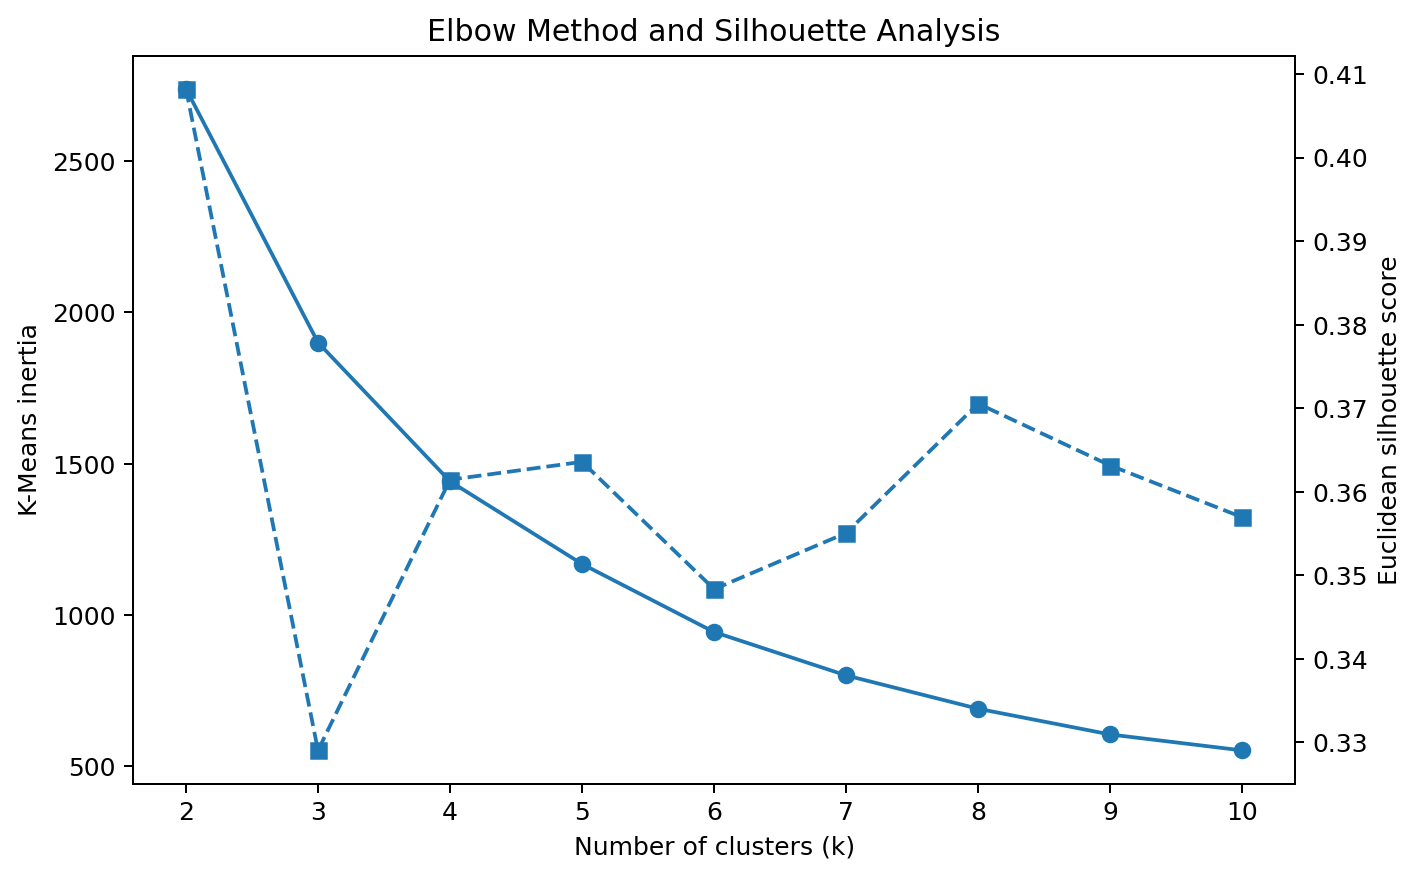
\includegraphics[width=\columnwidth]{01_elbow_silhouette.png}
\caption{K-Means inertia and Euclidean silhouette scores for $k=2$--$10$.}
\label{fig:elbow}
\end{figure}

\begin{table}[H]
\centering
\caption{Selected K-Means diagnostics.}
\label{tab:kdiag}
\footnotesize
\begin{tabular}{rcc}
\toprule
$k$ & Inertia & Silhouette\\
\midrule
2 & 2738.20 & \textbf{0.4082}\\
3 & 1900.03 & 0.3291\\
4 & 1441.61 & 0.3615\\
5 & 1168.49 & 0.3636\\
6 & 943.87 & 0.3484\\
7 & 800.70 & 0.3551\\
8 & 690.52 & 0.3705\\
9 & 605.65 & 0.3631\\
10 & 553.05 & 0.3569\\
\bottomrule
\end{tabular}
\end{table}

\subsection{Comparison of clustering methods}
Table~\ref{tab:models} compares the three partitions. Ward agglomerative clustering has the highest Euclidean silhouette (0.4615) and the lowest Davies--Bouldin index (0.8936), suggesting the strongest compactness and separation under Euclidean geometry among the evaluated methods. K-Means obtains a Euclidean silhouette of 0.4082 and Davies--Bouldin index of 1.0664. The average-linkage cosine model has the highest cosine silhouette (0.5363), which is expected to be judged under its own distance metric; its Euclidean silhouette is 0.2956 and its Euclidean Davies--Bouldin index is 1.3412. Thus, the preferred method depends on the distance geometry used for evaluation. Ward is strongest on Euclidean metrics, while the cosine model is strongest on cosine silhouette.

\begin{table}[H]
\centering
\caption{Internal evaluation of clustering methods ($k=2$).}
\label{tab:models}
\footnotesize
\begin{tabularx}{\columnwidth}{Xccc}
\toprule
\textbf{Method} & \textbf{Silh. Euc.} & \textbf{Silh. Cos.} & \textbf{DBI Euc.}\\
\midrule
K-Means & 0.4082 & 0.2757 & 1.0664\\
Ward / Euclidean & \textbf{0.4615} & 0.1785 & \textbf{0.8936}\\
Average / Cosine & 0.2956 & \textbf{0.5363} & 1.3412\\
\bottomrule
\end{tabularx}
\end{table}

\subsection{PCA projection}
The first principal component explains 45.8\% of the standardised feature variance and the second explains 36.9\%. Together, the two components explain 82.7\% of the variance. Figure~\ref{fig:pca} shows the K-Means partition in this two-dimensional projection. The two groups are visibly differentiated along the first component, although some overlap remains. The plot supports the existence of broad differences in seasonal profiles, but does not establish a geographic boundary or a causal explanation for the grouping.

\begin{figure}[H]
\centering
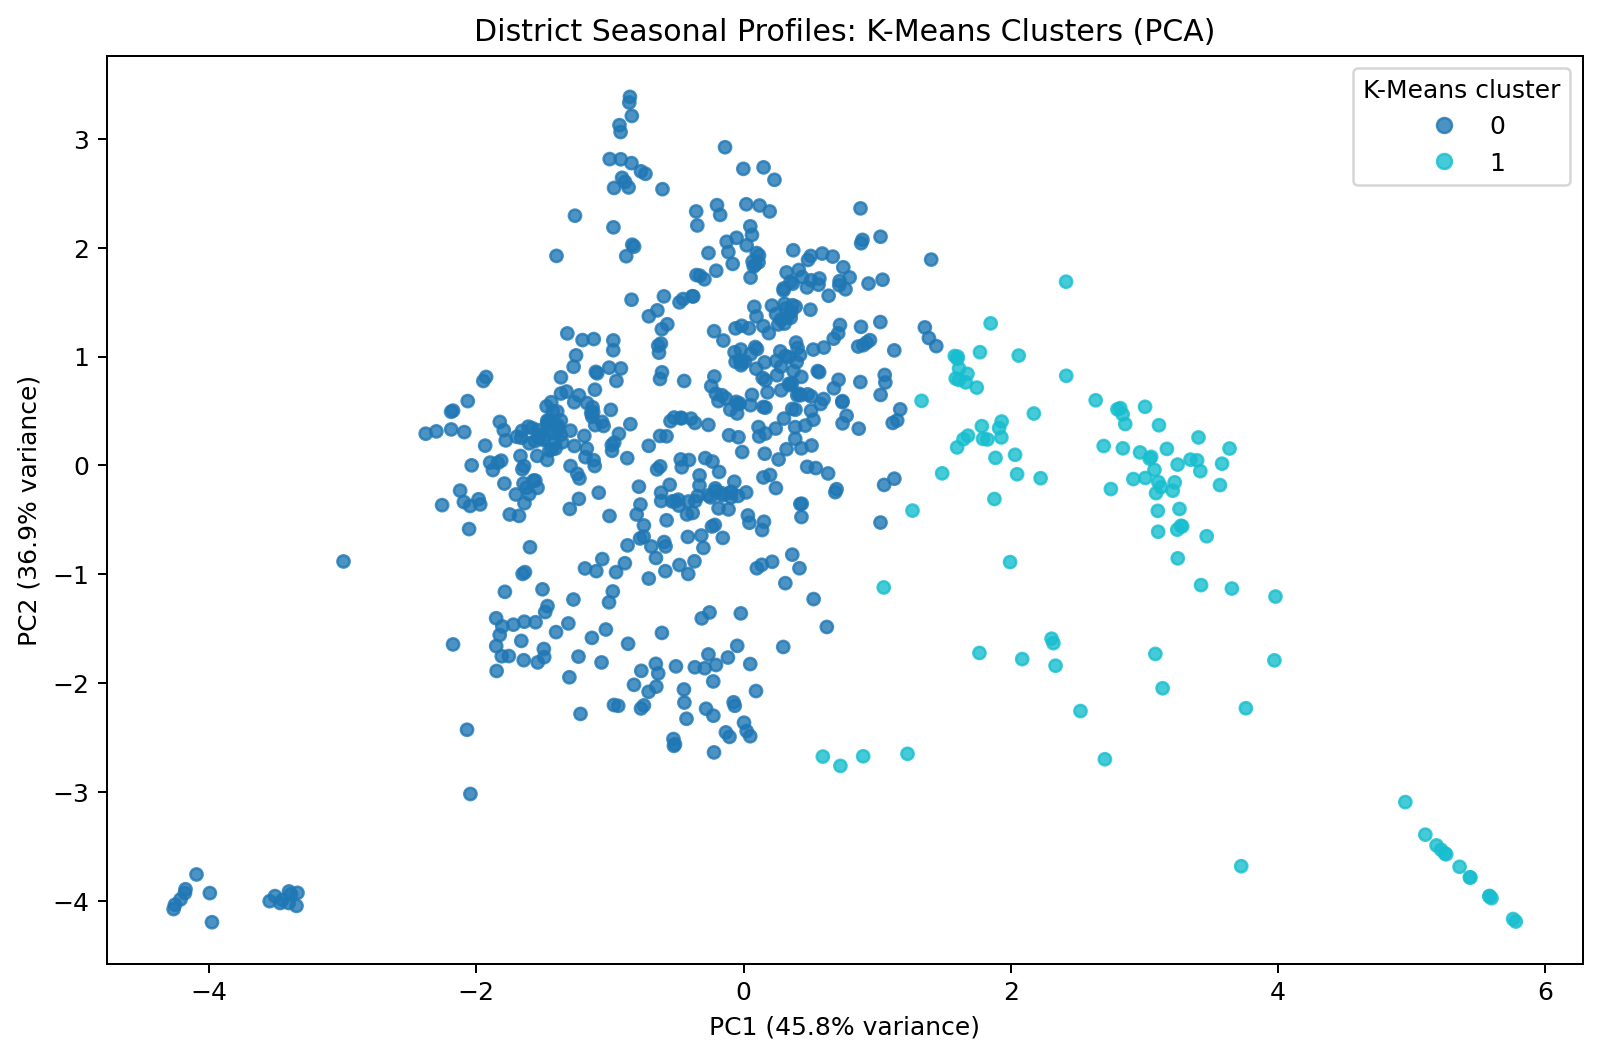
\includegraphics[width=\columnwidth]{02_pca_clusters.png}
\caption{PCA projection of the 643 district profiles, coloured by K-Means cluster. PC1 explains 45.8\% and PC2 36.9\% of the variance.}
\label{fig:pca}
\end{figure}

\subsection{Cluster profiles}
The K-Means solution contains 538 districts in Cluster 0 and 105 districts in Cluster 1. Cluster 0 has mean area shares of 52.3\% Kharif, 40.5\% Rabi and 7.2\% Whole Year. Its crop-balanced production-composition shares are 45.1\% Kharif, 32.1\% Rabi and 22.9\% Whole Year. This group is therefore described as a Kharif--Rabi area profile. Cluster 1 has mean area shares of 54.1\% Kharif, 4.9\% Rabi and 40.9\% Whole Year, with crop-balanced production-composition shares of 28.6\%, 10.9\% and 60.5\%, respectively. It is described as a Kharif--Whole Year area profile. These labels are descriptive summaries of cluster means, not official agricultural classifications.

\begin{table}[H]
\centering
\caption{Mean seasonal shares and district counts for K-Means clusters.}
\label{tab:profiles}
\scriptsize
\begin{tabular}{lrrr}
\toprule
\textbf{Feature} & \textbf{All} & \textbf{C0} & \textbf{C1}\\
\midrule
District count & 643 & 538 & 105\\
Area: Kharif & -- & 0.523 & 0.541\\
Area: Rabi & -- & 0.405 & 0.049\\
Area: Whole Year & -- & 0.072 & 0.409\\
Production*: Kharif & -- & 0.451 & 0.286\\
Production*: Rabi & -- & 0.321 & 0.109\\
Production*: Whole Year & -- & 0.229 & 0.605\\
\bottomrule
\end{tabular}
\vspace{1pt}\par\raggedright\scriptsize *Crop-balanced seasonal production-composition feature; not aggregate district tonnage share.
\end{table}

\begin{figure}[H]
\centering
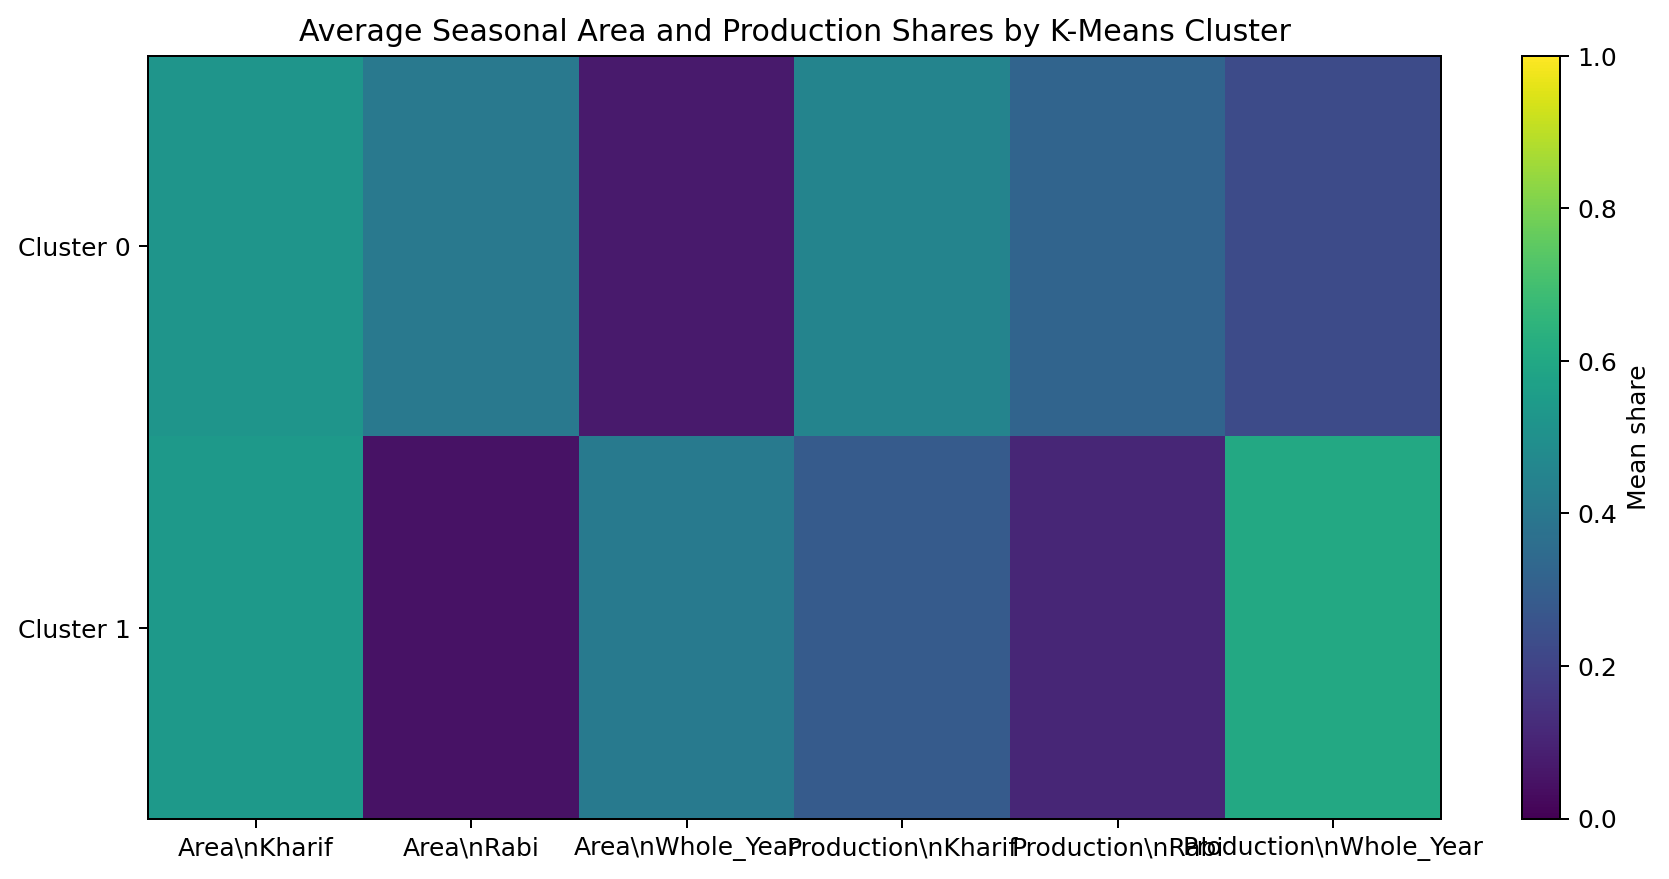
\includegraphics[width=\columnwidth]{03_cluster_profiles.png}
\caption{Mean area and crop-balanced production-composition shares for the two K-Means clusters.}
\label{fig:profiles}
\end{figure}

\section{Discussion}
The analysis identifies two broad seasonal-profile groups among the 643 retained district units. The larger group is characterised by area distributed mainly across Kharif and Rabi, while the smaller group has a substantial Whole Year area share alongside Kharif. Their production-composition profiles differ as well: Cluster 1 has a larger mean Whole Year crop-balanced production share, whereas Cluster 0 has higher Kharif and Rabi production-composition shares. This contrast suggests that seasonal area allocation and crop-level production composition provide complementary information about district agricultural profiles.

The Ward model performs best on Euclidean internal metrics, while the cosine model performs best on cosine silhouette. This is not a contradiction: Euclidean distance is sensitive to magnitudes in the standardised feature space, whereas cosine distance emphasises the direction or relative shape of feature vectors. The choice of clustering method should therefore depend on the intended interpretation. For the main district profiles, K-Means is retained because it provides a simple centroid-based partition and directly supports the cluster-mean profile table; the Ward result is reported as the strongest Euclidean benchmark.

The findings are consistent with the broader argument that Indian cropping patterns vary spatially and should be examined below the national scale [2,3]. However, the current features contain only seasonal area and crop-balanced production composition. They do not include rainfall, irrigation, soil, temperature, market access, farm size or yield. As a result, a cluster should not be interpreted as a causal agro-climatic zone or as proof that districts need identical interventions. The clusters can instead be used as an initial screening layer for further local investigation.

\subsection{Implications for SDGs}
The work is connected to SDG 2 (Zero Hunger), particularly the broad objective of supporting productive and sustainable agriculture, because a clearer description of seasonal crop patterns can help planners investigate where extension services and crop-related support may need to differ. It is also connected to SDG 15 (Life on Land), since understanding crop composition and seasonal land-use patterns can contribute to further assessments of agricultural diversity and sustainable land management. The present study does not directly measure food security, biodiversity, soil health or land degradation; therefore, its SDG contribution is indirect and informational rather than an evaluated impact.

\subsection{Limitations}
First, the 2015 records are markedly incomplete relative to earlier years and are excluded, so the analysis does not describe the latest agricultural conditions. Second, only three of the six source season labels are included, as required by the allocated problem; this omits Summer, Winter and Autumn patterns. Third, the production feature is an equally weighted average of crop-specific seasonal proportions. It deliberately prevents dominant crops from overwhelming the district signature, but it is not the aggregate production share by season and should be interpreted accordingly. Fourth, administrative district boundaries and names may have changed during 1997--2014; the supplied file does not provide stable district codes or historical boundary harmonisation. Fifth, internal clustering metrics cannot establish whether the resulting groups are useful to farmers or administrators. Finally, the dataset does not include explanatory variables such as rainfall, irrigation, soil characteristics or market access.

\section{Conclusion and Future Work}
This case study applied K-Means and agglomerative hierarchical clustering to six seasonal area and crop-balanced production-composition features for 643 Indian district units. The maximum Euclidean silhouette among the tested K-Means values occurred at $k=2$ (0.4082). Ward clustering produced the strongest Euclidean internal metrics (silhouette 0.4615; Davies--Bouldin 0.8936), while average-linkage cosine clustering achieved a cosine silhouette of 0.5363. The K-Means profiles distinguished a larger Kharif--Rabi area group and a smaller Kharif--Whole Year area group. These results offer a descriptive starting point for identifying districts with similar seasonal crop profiles. Future work should incorporate complete and updated district-level records, harmonised district identifiers, meteorological and irrigation variables, and validation with agricultural experts and local extension agencies. A geographic map and stability analysis across time periods would also help assess whether the groups are spatially coherent and persistent.

\section*{Declarations}
\noindent\textbf{Data availability.} The study uses the supplied crop-production CSV mirror of the Government of India's district-wise, season-wise crop-production statistics. The official resource is available at \smallurl{https://www.data.gov.in/resource/district-wise-season-wise-crop-production-statistics-1997}; the Kaggle mirror listed in the project allocation is \smallurl{https://www.kaggle.com/datasets/abhinand05/crop-production-in-india}. The analysis file used for the reported results is included with the project materials.

\noindent\textbf{Code availability.} The Jupyter Notebook, source CSV and LaTeX source are included with the assignment materials. The notebook uses a fixed random seed and writes its tables and figures to the project folder for reproducibility.

\noindent\textbf{Conflict of interest.} The author declares no conflict of interest.

\noindent\textbf{Funding.} No external funding was received for this academic assignment.

\noindent\textbf{Use of AI tools.} AI assistance was used in drafting and code-development support. The student should review the notebook, verify the outputs, understand the methodology and revise this declaration to accurately describe the tools used and the student's own contribution, in accordance with the college's academic-integrity rules.

\section*{References}
\begin{enumerate}[label={[\arabic*]},leftmargin=2.2em,itemsep=4pt]
\item Directorate of Economics and Statistics, Department of Agriculture and Farmers Welfare, Ministry of Agriculture and Farmers Welfare, Government of India, ``District-wise, season-wise crop production statistics from 1997,'' Open Government Data Platform India. [Online]. Available: \smallurl{https://www.data.gov.in/resource/district-wise-season-wise-crop-production-statistics-1997}. Accessed: 03-Nov-2026. The OGD catalogue describes the underlying resource as district-, crop-, season- and year-wise area and production statistics.
\item J. C. Smith, A. Ghosh, and R. J. Hijmans, ``Agricultural intensification was associated with crop diversification in India (1947--2014),'' \textit{PLOS ONE}, vol. 14, no. 12, e0225555, 2019, doi: 10.1371/journal.pone.0225555.
\item ``Climate change and transition in cropping patterns: District level evidence from West Bengal, India,'' \textit{Environmental Challenges}, vol. 7, Art. no. 100499, 2022, doi: 10.1016/j.envc.2022.100499.
\item J. MacQueen, ``Some methods for classification and analysis of multivariate observations,'' in \textit{Proc. Fifth Berkeley Symp. Math. Statistics and Probability}, vol. 1, 1967, pp. 281--297.
\item J. H. Ward, Jr., ``Hierarchical grouping to optimize an objective function,'' \textit{Journal of the American Statistical Association}, vol. 58, no. 301, pp. 236--244, 1963, doi: 10.1080/01621459.1963.10500845.
\item P. J. Rousseeuw, ``Silhouettes: A graphical aid to the interpretation and validation of cluster analysis,'' \textit{Journal of Computational and Applied Mathematics}, vol. 20, pp. 53--65, 1987, doi: 10.1016/0377-0427(87)90125-7.
\item D. L. Davies and D. W. Bouldin, ``A cluster separation measure,'' \textit{IEEE Transactions on Pattern Analysis and Machine Intelligence}, vol. PAMI-1, no. 2, pp. 224--227, 1979, doi: 10.1109/TPAMI.1979.4766909.
\item I. T. Jolliffe, \textit{Principal Component Analysis}, 2nd ed. New York, NY, USA: Springer, 2002.
\item F. Pedregosa et al., ``Scikit-learn: Machine learning in Python,'' \textit{Journal of Machine Learning Research}, vol. 12, pp. 2825--2830, 2011.
\end{enumerate}

\section*{Appendix A. Cluster profile summary}
Table~\ref{tab:profiles} provides the numerical cluster profiles used for interpretation. Cluster identifiers (0 and 1) are arbitrary algorithmic labels and do not indicate rank or quality. The following short descriptions are intended only as convenient summaries of the mean seasonal shares:
\begin{itemize}
\item \textbf{Cluster 0 (538 districts):} Kharif--Rabi area profile; mean area shares are 52.3\% Kharif, 40.5\% Rabi and 7.2\% Whole Year.
\item \textbf{Cluster 1 (105 districts):} Kharif--Whole Year area profile; mean area shares are 54.1\% Kharif, 4.9\% Rabi and 40.9\% Whole Year.
\end{itemize}
The complete district-to-cluster assignments, PCA coordinates, model evaluation table and cluster-profile CSV are provided alongside the notebook for reproducibility.

\end{document}
